\chapter{Geometria Plana}

\section{Áreas e Perímetros}

\quest{Guarda Metropolitano Prefeitura de Palmas TO - VUNESP 2023}{Em um terreno retangular ABCD, com 30 m de largura por 50 m de comprimento, foi construída uma arquibancada, banheiros (W) e vestiários, todos retangulares, conforme mostra a figura. O espaço livre foi destinado à construção de uma quadra poliesportiva.
\begin{center}
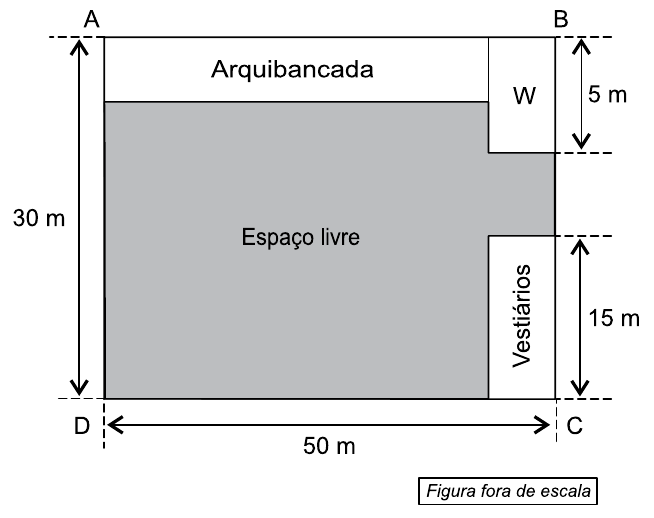
\includegraphics[scale=.5]{fig004.png}
\end{center}
Sabendo que as áreas do vestiário, da arquibancada e dos banheiros são, respectivamente, iguais a 30 m², 144 m² e 10 m², então, o perímetro do espaço livre, destacado na figura, é igual a}{
\item 168 m.
\item 165 m.
\item 160 m.
\item 154 m.}
{https://youtu.be/hcdlzi_qYfc}


\section{Teorema de Pitágoras}
\quest{Transpetro 2023 - CESGRANRIO}{O triângulo ABC é retângulo em A. Sabe-se que o comprimento da hipotenusa BC é igual a 20 cm, e que o comprimento do cateto AB é igual a 12 cm. Qual é a área, em cm², do triângulo ABC?
}
{
\item 16
\item 48
\item 60
\item 96
\item 240}
{https://youtu.be/YP9XL4Pdrik}

